\section{Introduction}
Large language models (LLMs) such as GPT-3.5~\cite{brown2020language}, GPT-4~\cite{achiam2023gpt}, and PaLM 2~\cite{anil2023palm} are widely deployed in the real world for their exceptional generative capabilities.
Despite their success, they also have inherent limitations. For instance, they lack up-to-date knowledge as they are pre-trained on past data (e.g., the cutoff date for the pre-training data of GPT-4 is April 2023~\cite{achiam2023gpt}); they exhibit hallucination behaviors~\cite{ji2023survey} (e.g., generate inaccurate answers);
they could have gaps of knowledge in particular domains (e.g., the medical domain). 
These limitations pose severe challenges for deploying LLMs in many real-world applications in healthcare~\cite{al2023transforming, wang2023potential}, finance~\cite{loukas2023making}, law~\cite{kuppa2023chain, mahari2021autolaw}, and scientific research~\cite{kumar2023mycrunchgpt, boyko2023interdisciplinary, prince2023opportunities} fields.


\begin{figure}[!t]
	 \centering
{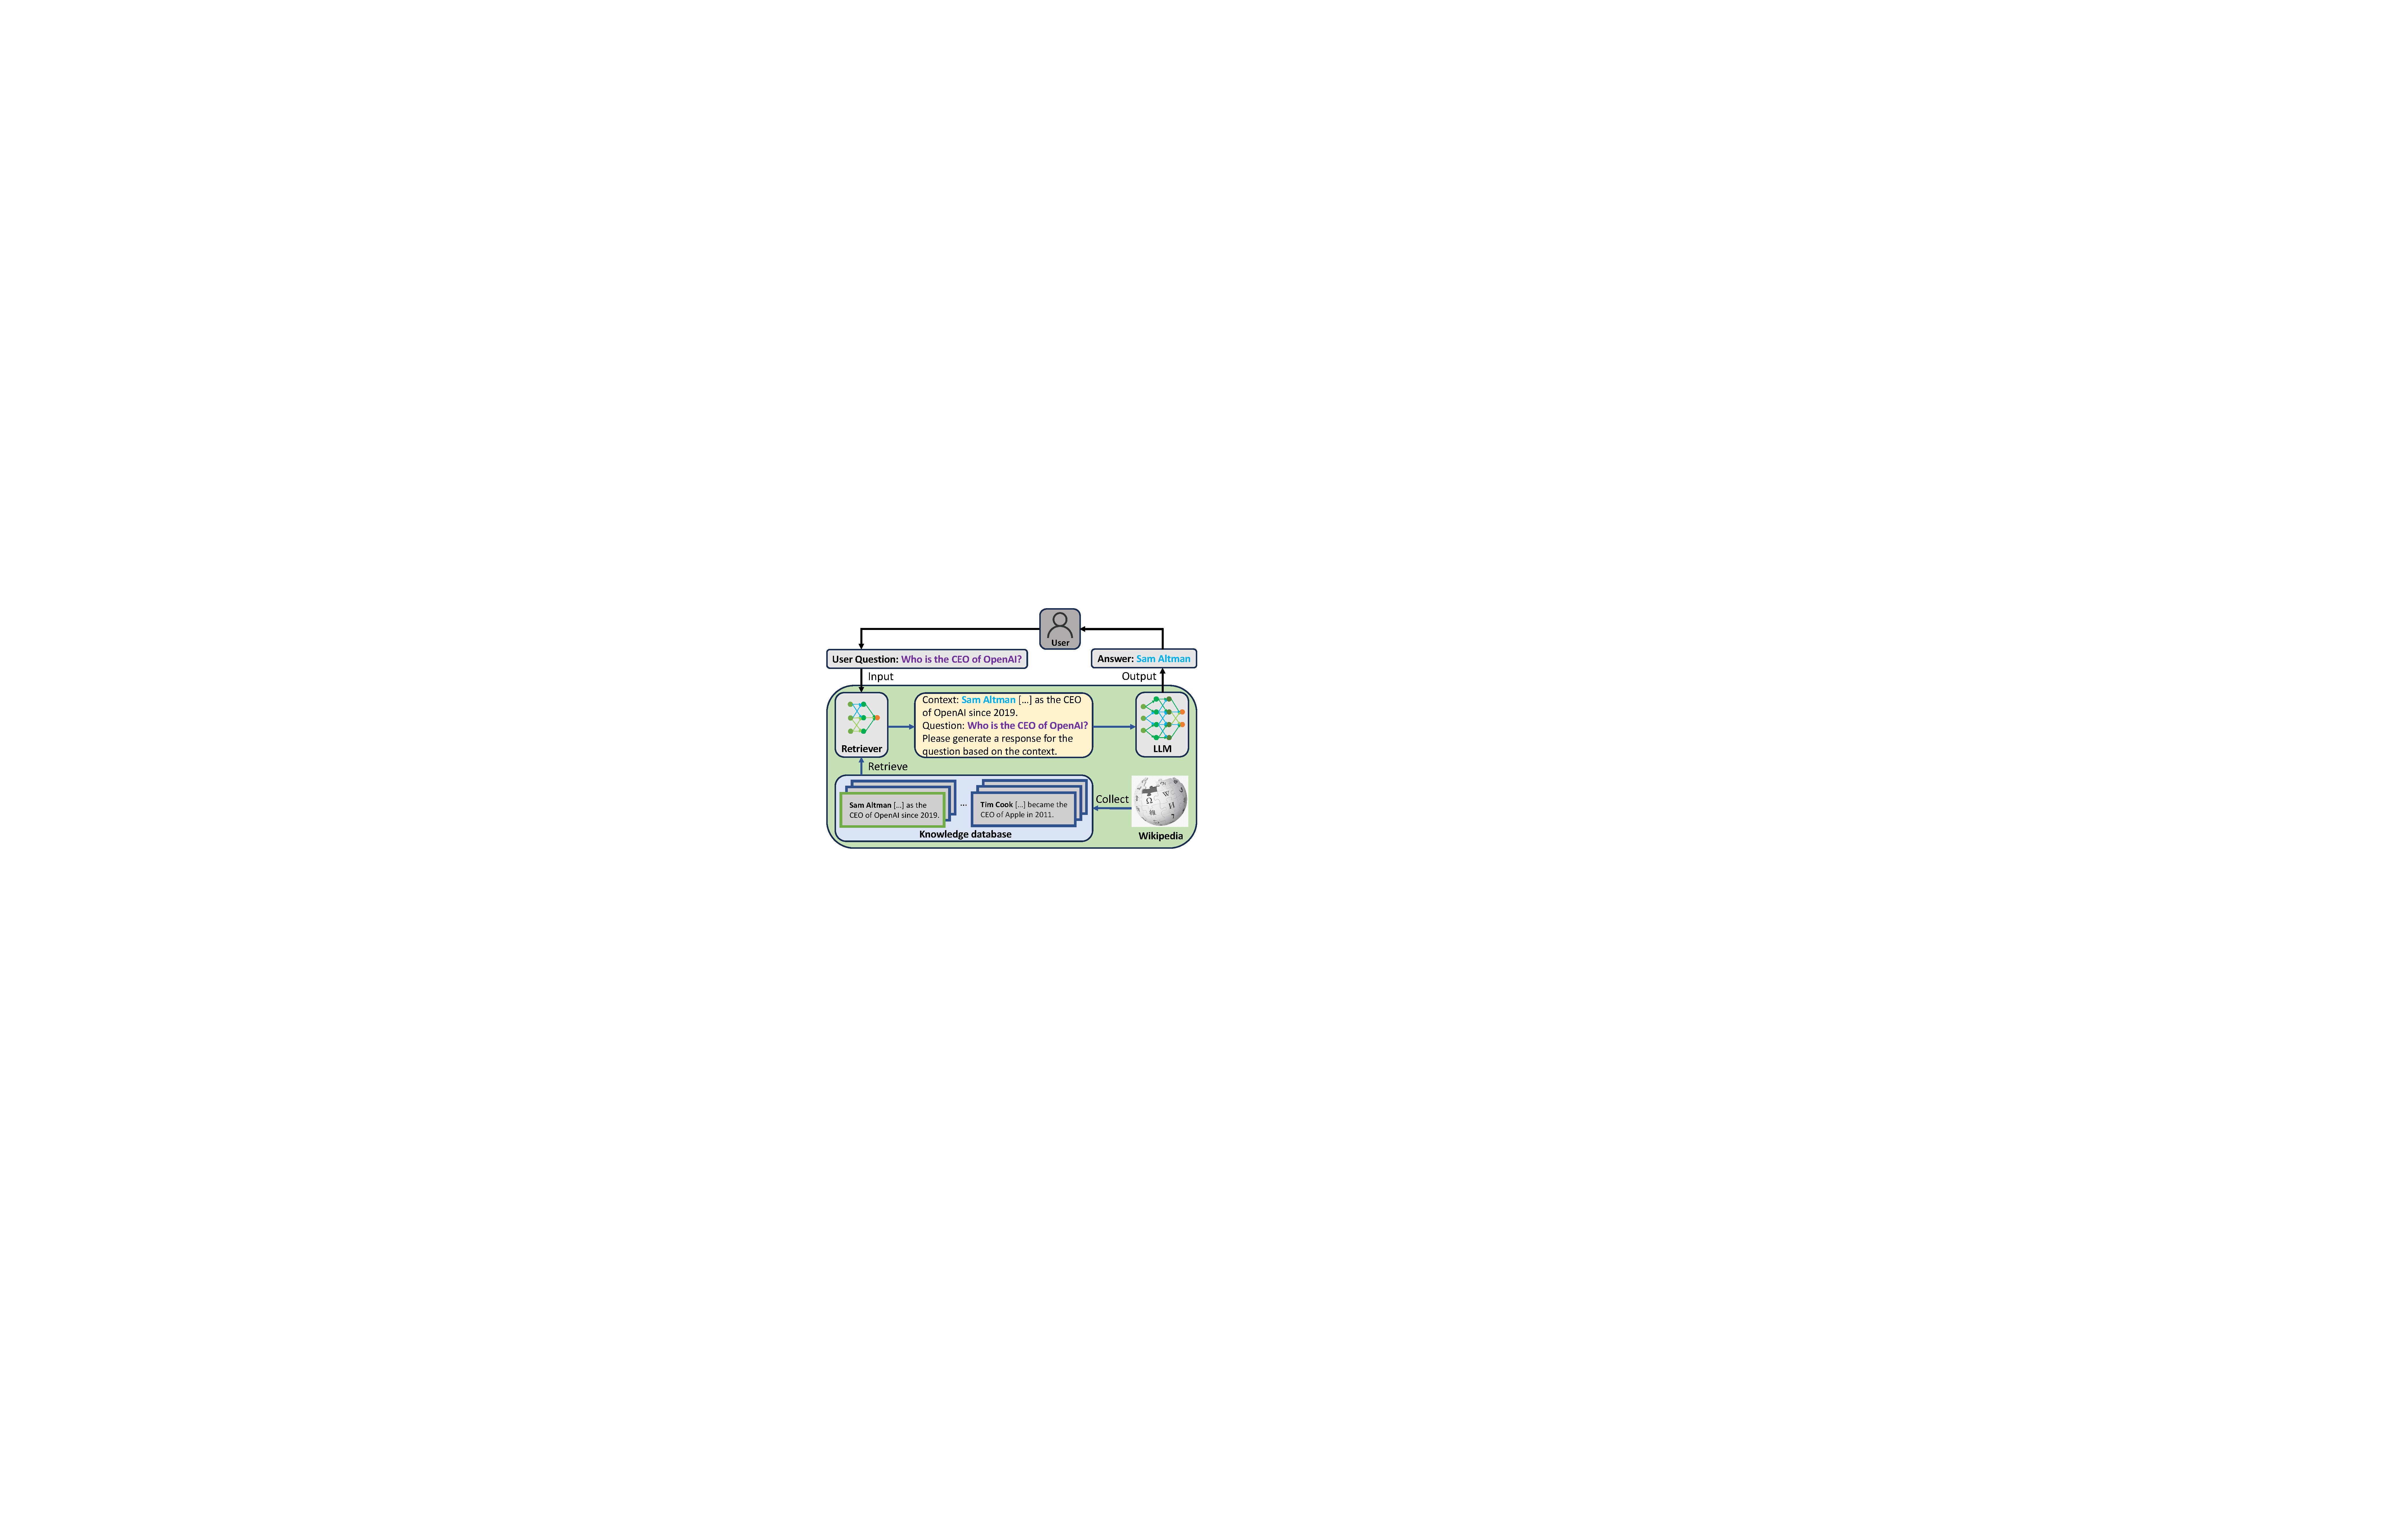
\includegraphics[width=0.48\textwidth]{figs/RAG.pdf}}
\caption{Visualization of RAG.}
\label{rag-demo}
\vspace{-6mm}
\end{figure}



\emph{Retrieval-Augmented Generation (RAG)}~\cite{karpukhin2020dense,lewis2020retrieval,borgeaud2022improving,thoppilan2022lamda} is a 
state-of-the-art technique to mitigate those limitations, which augments an LLM with external knowledge retrieved from a knowledge database. 
As shown in Figure~\ref{rag-demo}, there are three components in RAG: \emph{knowledge database}, \emph{retriever}, and \emph{LLM}. A knowledge database contains a large number of texts collected from various sources such as Wikipedia~\cite{thakur2021beir}, financial documents~\cite{loukas2023making}, news articles~\cite{soboroff2019trec}, COVID-19 publications~\cite{voorhees2021trec}, to name a few. 
A retriever is used to retrieve a set of most relevant texts from the knowledge database for a question.
With the help of a system prompt, the retrieved texts are used as the context for the LLM to generate an answer for the given question. 
RAG enables an LLM to utilize external knowledge in a plug-and-play manner. Moreover, RAG can reduce hallucinations and enhance the domain-specific expertise of an LLM.
Due to these benefits, we have witnessed a variety of developed tools (e.g., ChatGPT Retrieval Plugin~\cite{chatgpt-retrieval},
 LlamaIndex~\cite{Liu_LlamaIndex_2022}, ChatRTX~\cite{chat-with-rtx}, and LangChain~\cite{lang_chain}) and real-world applications (e.g., WikiChat~\cite{semnani-etal-2023-wikichat}, Bing Search~\cite{bing-search}, Clinfo.AI~\cite{lozano2023clinfo}, Google Search with AI Overviews~\cite{google-search-ai-overview}, Perplexity AI~\cite{perplexity-ai}, and LLM agents~\cite{shinn2023reflexion,yao2022react}) of RAG.


Existing studies~\cite{asai2023self, izacard2022unsupervised, xiong2021approximate, peng2023soft, kassner2020bert, karpukhin-etal-2020-dense} mainly focused on improving the accuracy and efficiency of RAG. For instance, some studies~\cite{izacard2022unsupervised, xiong2021approximate, karpukhin-etal-2020-dense} designed new retrievers such that more relevant knowledge could be retrieved for a given question. Other studies~\cite{asai2023self, peng2023soft, kassner2020bert} proposed various techniques to improve the efficiency of knowledge retrieval.
However, the security of RAG is largely unexplored.


To bridge the gap, we propose {\name}, the \emph{first} knowledge corruption attack to RAG. 


\noindent
\myparatight{Knowledge database as a new and practical attack surface} In this work, we find that knowledge databases of RAG systems introduce a new and practical attack surface. In particular, an attacker can inject malicious texts into the knowledge database of a RAG system to induce an LLM to generate attacker-desired answers to user questions. For instance, when the knowledge database contains millions of texts collected from Wikipedia, an attacker could inject malicious texts by maliciously editing Wikipedia pages~\cite{carlini2023poisoning}; an attacker could also post fake news or host malicious websites to inject malicious texts when the knowledge databases are collected from the Internet; an insider can inject malicious texts into an enterprise private knowledge database.



\myparatight{Threat model} 
 In {\name}, an attacker first selects one or more questions (called \emph{target questions}) and selects an arbitrary answer (called \emph{target answer}) for each target question. The attacker aims to inject malicious texts into the knowledge database of a RAG system such that an LLM generates the target answer for each target question. For instance, an attacker could mislead the LLM to generate misinformation (e.g., the target answer could be ``Tim Cook'' when the target question is ``Who is the CEO of OpenAI?''), commercial biased answers (e.g., the answer is a particular brand over others when asked for recommendations on consumer products), and financial disinformation about markets or specific companies (e.g., falsely stating a company is facing bankruptcy when asked about its financial situation).
 These attacks pose severe challenges for deploying RAG systems in many safety and reliability-critical applications such as cybersecurity, financial services, and healthcare. 

We consider an attacker cannot access texts in the knowledge database and cannot access/query the LLM in RAG. The attacker may or may not know the retriever. With it, we consider two settings: \emph{white-box setting} and \emph{black-box setting}. The attacker could access the parameters of the retriever in the white-box setting (e.g., a publicly available retriever is adopted in RAG), while the attacker cannot access the parameters nor query the retriever in the black-box setting. As mentioned before, we consider an attacker can inject a few malicious texts into a knowledge database of a RAG system. 




\myparatight{Overview of {\name}}We formulate crafting malicious texts as an optimization problem. However, it is very challenging to directly solve the optimization problem. In response, we resort to heuristic solutions that involve deriving two conditions, namely \emph{retrieval condition} and \emph{generation condition} for malicious texts that can lead to an effective attack. The retrieval condition means a malicious text can be retrieved for a target question. The generation condition means a malicious text can mislead an LLM to generate a target answer for a target question when the text is used as the context. 
We then design attacks in both white-box and black-box settings to craft malicious texts that simultaneously satisfy the two conditions. Our key idea is to decompose a malicious text into two sub-texts, which are crafted to achieve two conditions, respectively. Additionally, when concatenating the two sub-texts together, they simultaneously achieve these two conditions. 

\noindent
\myparatight{Evaluation of {\name}} We conduct systematic evaluations of {\name} on multiple datasets (Natural Question (NQ)~\cite{kwiatkowski2019natural}, HotpotQA~\cite{yang2018hotpotqa}, MS-MARCO~\cite{nguyen2016ms}), 8 LLMs (e.g., GPT-4~\cite{achiam2023gpt}, LLaMA-2~\cite{touvron2023llama}), and three real-world applications, including advanced RAG schemes, Wikipedia-based chatbot, and LLM agent. We use Attack Success Rate (ASR) 
as the evaluation metric, which measures the fraction of target questions whose answers are attacker-desired target answers under attacks. We have the following observations from our results. First, {\name} could achieve high ASRs with a small number of malicious texts. For instance, on the NQ dataset, we find that {\name} could achieve a 97\% ASR by injecting 5 malicious texts for each target question into a knowledge database (with 2,681,468 clean texts) in the black-box setting. Second, {\name} outperforms the SOTA 
baselines~\cite{liu2023prompt,zhong2023poisoning}. For instance, on the NQ dataset, {\name} (black-box setting) achieves a 97\% ASR, while ASRs of 5 baselines are less than 70\%.
Third, our ablation studies show {\name} is robust against different hyper-parameters.


\noindent
\myparatight{Defending against {\name}} We explore several defenses, including paraphrasing~\cite{jain2023baseline} and perplexity-based detection~\cite{jain2023baseline, alon2023detecting, gonen2022demystifying}. Our results show these defenses are insufficient to defend against {\name}, thus 
highlighting the need for new defenses. 

Our major contributions are as follows:
\begin{itemize}
\vspace{-1mm}
    \item We propose {\name}, the \emph{first} knowledge corruption attack that exploit the new attack surface introduced by knowledge databases of RAG systems. 
    \vspace{-1mm}
    \item 
    Our major contribution is to derive two necessary conditions for an effective attack to RAG systems. We further design {\name} to achieve these two conditions.
    \vspace{-1mm}
    \item We conduct an extensive evaluation for {\name} on multiple knowledge databases, retrievers, RAG schemes, and LLMs. Additionally, we compare {\name} with 5 baselines. 
    \vspace{-1mm}
    \item We explore several defenses against {\name}. 
\end{itemize}

